% Allow relative paths in included subfiles that are compiled separately
% See https://tex.stackexchange.com/questions/153312/

\providecommand{\main}{..}
\documentclass[\main/thesis.tex]{subfiles}
\externaldocument{}


\begin{document}
\chapter{Representing Sound}
\section{Feature Selection}

Throughout the project, we will work with 1 second sounds snippets made with synthesizers with stack sizes of 8 or fewer. Even with these constraints, the set of possible synthesizer parameters---and we assume, the sound generated by the synth given these parameters---is extremely large. Additionally, as discussed in Section~\ref{surveys}, the majority of sounds generated by the synth do not resemble percussion.  We believe there are 2 steps necessary to effectively extract percussive sounds
from the randomly generated sounds produced by virtual synthesizers: 
\begin{enumerate}
   \item Phase $1$: Binary separation of sounds with percussive features from non-percussive sounds.
   \item Phase $2$: Given confidence that the sound being categorized is percussive, categorizing its type.
\end{enumerate}
We are interested in extracting generalizable, domain agnostic features to train our virtual ear models. We can facilitate the learning process by representing sounds in a small feature space without the loss of critical information.

\section{Fourier Transforms}
In this work we rely on derivatives of the fast Fourier transform (FFT) and by extension short-time Fourier transforms (STFT) for feature extraction. Using FFT, a signal can be represented by a vector with each index corresponding to a frequency-bin (a range of frequencies too close to be distinguishable) and the value at each index corresponding to the combined-magnitude of the frequencies within the bin. STFT can be employed when a more accurate representation is desired; via the application of the FFT to a sliding time-window on the signal to create a matrix (a list of vectors). This matrix can effectively represent the frequencies present in the signal at each time step, given the right window-length and hop-size (how much the window is shifted at each time-step).
\begin{figure}
\centering
\textbf{Visual Representation of Raw Features}\par\medskip
    \subcaptionbox{Recorded hat sample}{    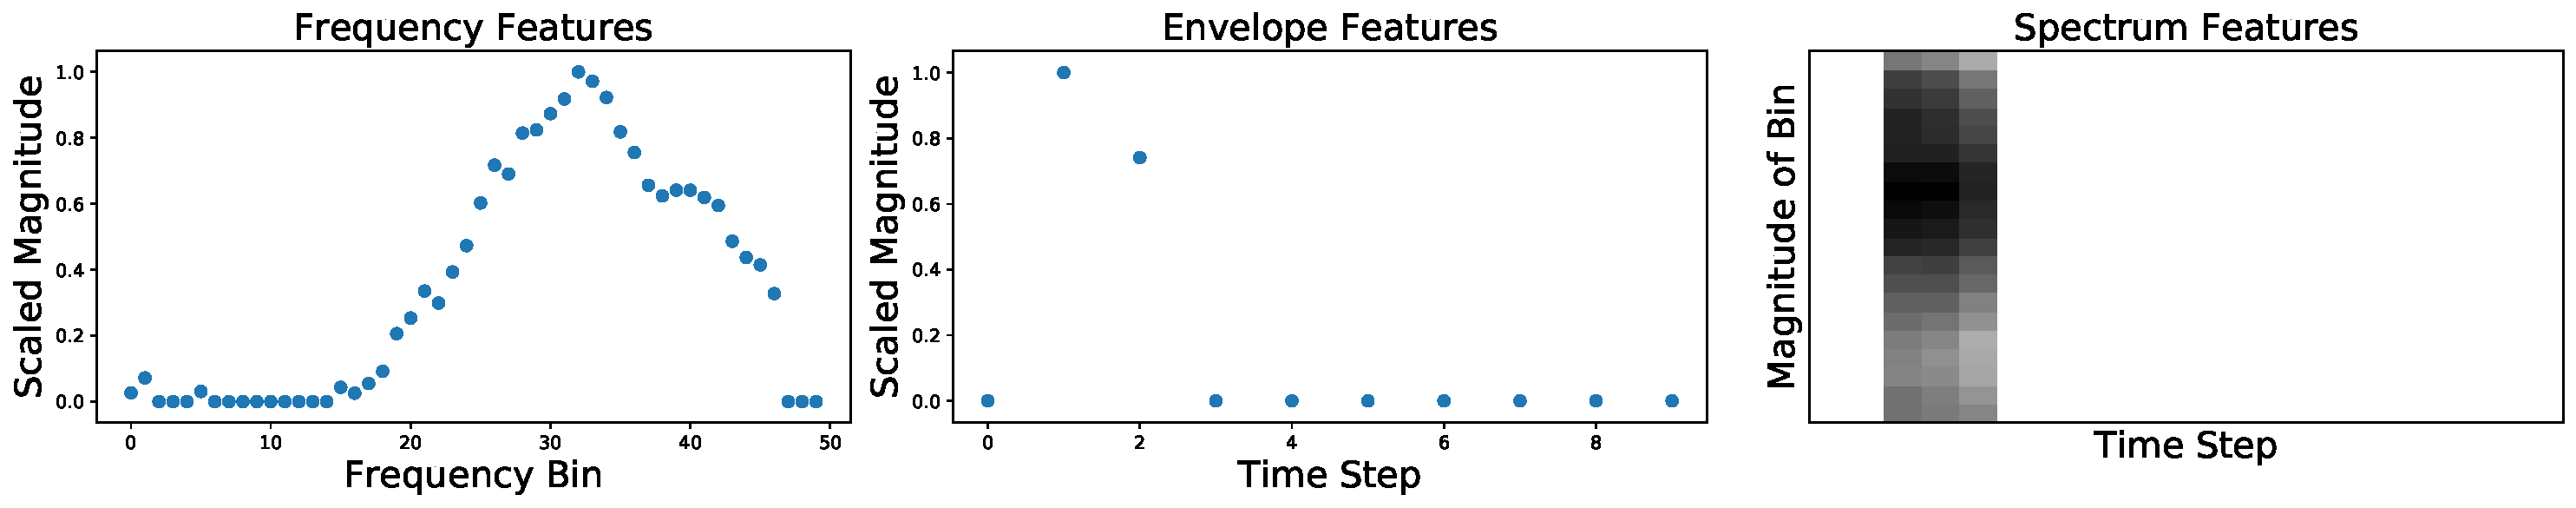
\includegraphics[width=1\columnwidth]{images/ff1.pdf}
    }
    \subcaptionbox{Randomly generated audio with percussive qualities, resembling a tight snare}{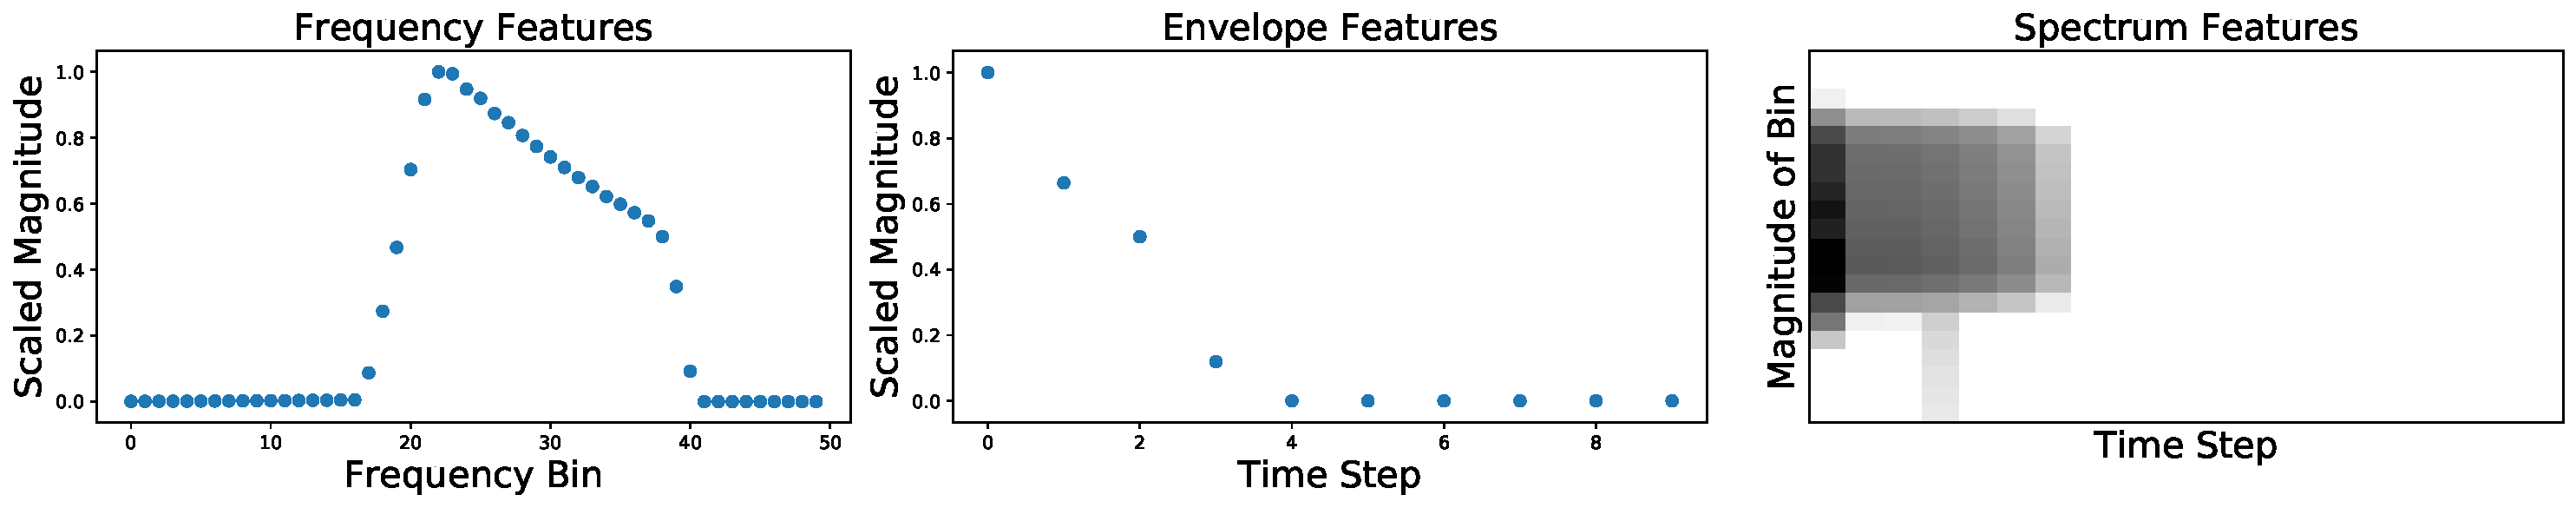
\includegraphics[width=1\columnwidth]{images/ff2.pdf}}
    \subcaptionbox{A randomly generated noise with a percussive envelop but non-percussive frequency features (modulated pitch)}
    { 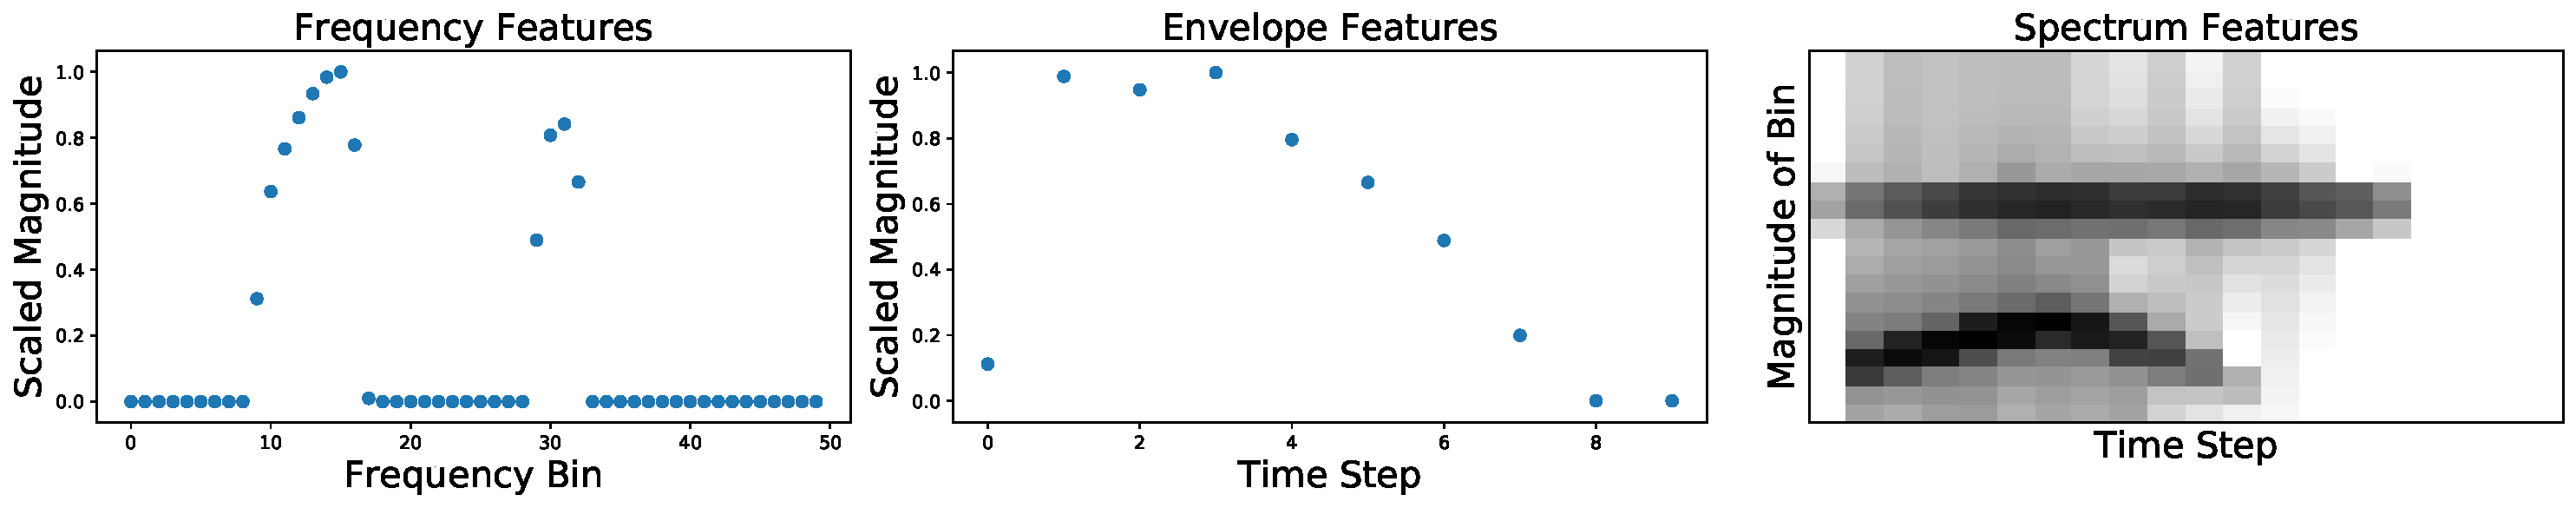
\includegraphics[width=1\columnwidth]{images/ff3.pdf}}
\caption{Graphed representation of features extracted for 3 different samples. Sample $a$ is a recorded hat from our database. sample $b$ is an example of randomly generated noise with percussive qualities that we found suitably similar to a snare sound. Sample $c$ is an example of a randomly generated noise where the spectrum features are necessary for proper classification.}
\label{fig:stackspectrums}
\end{figure}

Various works have demonstrated effective reconstruction of signals given their STFT~\cite{nawab1983signal,griffin1984signal}. For our purpose, if the original signal can be faithfully reconstructed from its STFT, analysis of the STFT may be relied on as source of fundamental features necessary for audible signal categorization. In the interest of keeping the feature space small and fundamental, other methods of feature extraction such as Spectral-Centroids~\cite{schubert2004spectral} and Zero-Crossing Rates~\cite{gouyon2000use} are not utilized.

Using only the STFT of signals as source of feature extraction we defined 3 transformation functions which we believe to capture important, unique attributes of percussive sounds.  These functions were applied at training time to 1 second audio samples before being sent to a classifier; transforming a signal into a set of features which we hope can capture the necessary information for our categorization task. 


\begin{enumerate}
\item Envelope Transformation: The goal of this feature is to capture the changes in loudness for the duration of the signal. Using STFT we generate a matrix $M_{i \times j}$ with rows $i$ and columns $j$ corresponding to time steps and frequency bins respectively, and with values $v_{i \times j}$ indicating the magnitude of the frequency bin $j$ at each time-step $i$. Information about the envelope of the signal can be extracted by summing the values of $M$ for each time-step (or row $i$), giving us a feature vector $v_i$. This vector is then normalized to the range of 0 to 1. The information contained in this vector is similar to that of a Root-Mean-Square measurement.
\item Frequency Transformation: A static, normalized snap-shot of the the frequencies present within the audio. The calculation of this feature vector is similar to the envelope, but the summation is done along the frequency axis. Another important distinction is that since capturing an adequate frequency resolution is important for this transformation, we utilized shorter hop-sizes and wider windows. A Mel Scale transformation was also applied in hopes that the captured features better represent human perception of frequencies. 
\item Spectrum Transformation: This function is simply a Mel Scaled STFT with its values normalized from 0-1. Since this features is a 2D matrix rather than a vector it captures more information about our signal but requires heavier, more complex computational methods to be utilized. 
\end{enumerate}


\section{Embedding Ears}
% http://www.justinsalamon.com/uploads/4/3/9/4/4394963/cramer_looklistenlearnmore_icassp_2019.pdf says they need almost 40 million samples 
% http://www.cs.toronto.edu/~zemel/documents/prototypical_networks_nips_2017.pdf
% 
Like many other categorization tasks, we seek features that capture critical information about our data in the most compact format possible. Feature extraction is a form of dimensionality reduction. While manual definition of the desired features can yield results, we also trained various autoencoder networks to encode our spectral features without supervision. 

As discussed previously in Section \ref{bg:NN}, many variations and applications of deep autoencoder networks have been proposed since Hinton et al. demonstrated effective dimensionality reduction via deep autoencoder networks \cite{hinton1994autoencoders,hinton2006reducing}. Particularly relevant are recent works by Aouameur et al. and Ramires et al. which influence the output of generative neural networks used for the synthesis of percussive sounds by inputting the low dimensional representation of desired traits \cite{aouameur2019neural,ramires2020neural}. 

We designed a number of autoencoder networks for the purpose of extracting features from our dataset of drum samples. Auto-encoders are comprised of an encoder and a decoder. The encoder has the task of meaningfully projecting the spectrum data of each sound into a small bottleneck layer, while the decoder aims to use this projection to replicate the input data as closely as possible. Successful training will lead to an encoder network capable of projecting audio data into a low dimensional vector, in other words, a feature extractor. 

We kept our autoencoder designs relatively simple, all with approximately 150,000 parameters. Important to mention is that reported loss values of the model do not reflect whether the encoder will capture data that is useful for any purpose other than being utilized by the decoder. Also important is that we do not give any examples of synthetic noise to the encoders, and only train on organic drums. We hope that if a synthetic noise has drum-like characteristics, its compressed, latent representation given by the encoder will be similar to those of drum sounds and vice versa. We then use these latent expressions to train a support vector machine (SVM) model.
\begin{table}[h!]

\begin{tabular}{|p{28mm}|p{50mm}|p{21mm}|p{21mm}|}
\hline
Hyper-Param. & Description  & Values & Distribution\\ \hline
Model Type      &   Affects encoder's first hidden layer & CNN,FC & Categorical \\  \hline
Optimizer       & Updates network's weights based on loss & Adam,SGD & Categorical  \\  \hline
Hidden Layers   & Extra hidden layer for the Encoder & True,False & Categorical \\  \hline
Time Steps & Temporal granularity of the spectrogram. Affects FFT windowing. & 10,20 & Categorical  \\ \hline
Learning Rate   &    Optimizer's learning rate  & $1^{-4}$ ... $1^{-1}$ & Uniform      \\ \hline
Frequency Bins & Number of spectrogram frequency bins & 10, 30,60 & Categorical \\ \hline

Regularization  &  L2 regularization parameter. Penalizes large weights to prevent overfitting & 1^{-6}~...~1^{-1} & Uniform\\ \hline
Latent Size & Size of bottle neck layer or number encoded features & 8,16,64 & Categorical              \\ \hline
Dropout Rate & Random zeroing of activations between layers to prevent over-fitting & 0,0.5,0.1 & Categorical\\  \hline
\end{tabular}
\caption{The Hyper-Paramter space in which the optimization was conducted.}
\label{table:hyper_params}
\end{table}

\subsection{Architecture and Hyper-Parameter Optimization}
% could do multi-objective pareto front stuff

Within the context of machine learning, a model's \emph{hyper-parameters} are fixed parameters which are set before the training begins (e.g number of layers, size of layers, loss function) and are not learned during the minimization procedure~\cite{bengio2000gradient}. Also within this context, hyper-parameter optimization is the task of searching for a set of hyper-parameters which would maximize the model's capacity, often done by a series of automatic test trials~\cite{bengio2000gradient,bergstra2011algorithms,bergstra2012random}. As a wide variety of viable autoencoder architectures have been proposed~\cite{aouameur2019neural,esling2018generative,gensler2016deep,zhang2016facing,pu2016variational}, we are faced with a number of choices for autoencoder design. To assist us with the construction of our model, we defined a number of possible choices for the architecture of our model and audio-transformers and used hyper-parameter optimization to extract promising sets of values~\ref{table:hyper_params}. 

The list of possible choices for the selected hyper-parameters can be found in table~\ref{table:hyper_params}. The batchsize, $\mathcal{B}$, was set to 64 for training and 4 for testing. We included not only model parameters but also spectrogram transformation parameters within this search space, as GPU accelerated FFT calculations allows ad hoc audio transformations to take place parallel to the training process. We implemented 3 base models which are affected by these hyper-parameters. The \enquote{Model Type} parameter dictates whether CNN or fully connected models are selected; If a \enquote{fully connected} model is selected, the \enquote{hidden layers} parameter selects between the two implementations. The specifications for these models can be found in tables~\ref{table:FC1_AUTOENCODER},~\ref{table:FC2_AUTOENCODER} and~\ref{table:CNNAUTOENCODER}.

\begin{table}[h]
\begin{tabular}{|p{28mm}|p{25mm}|p{23mm}|p{50mm}|}
\hline
Layer-\# & Out Shape & Param Num & Details  \\ \hline
Conv2d-1 & [$\mathcal{B}$, 8, 30, 20] &   208 & Encoder's input \newline
Num. Channels:8\newline
kernel:5x5\newline                  
stride:1\newline    
padding:2 \\ \hline
ReLU-2 & [$\mathcal{B}$, 8, 30, 20] &   0 & \\  \hline
MaxPool2d-3 & [$\mathcal{B}$, 8, 15, 10] & 0 &  kernel:5x5 \newline
stride:2 \\ \hline
Dropout-4 & [$\mathcal{B}$, 8, 15, 10] & 0 &  \\ \hline
Linear-5 & [$\mathcal{B}$, 8] & 9,608 & Encoder's output \\ \hline
Linear-6 & [$\mathcal{B}$, 256] & 2,304 & Decoder's Input \\ \hline
Dropout-7 & [$\mathcal{B}$, 256] & 0 &  \\ \hline
Linear-8 & [$\mathcal{B}$, 600 ] &  154,200& Decoder's output\\ \hline
\end{tabular}
\caption{CNN model design with latent size of 8. 30 and 20 are the assumed frequency bins and step size. Total number of parameters is 166,320. }
\label{table:CNNAUTOENCODER}
\end{table}

\begin{table}[h]
\begin{tabular}{|p{28mm}|p{25mm}|p{23mm}|p{50mm}|}
\hline
Layer-\# & Out Shape & Param Num & Details  \\ \hline
Linear-1 & [$\mathcal{B}$, 128]  & 76,928 & Encoder's input \\ \hline
Dropout-2 & [$\mathcal{B}$, 128] & 0 &  \\ \hline
Linear-3 & [$\mathcal{B}$, 8] & 9,608 & Encoder's output \\ \hline
Linear-4 & [$\mathcal{B}$, 128] & 2,304 & Decoder's Input \\ \hline
Dropout-5 & [$\mathcal{B}$, 128]  & 0 &  \\ \hline
Linear-6  & [$\mathcal{B}$, 600 ] &  77,400 &Decoder's output\\ \hline
\end{tabular}
\caption{Fully connected model with only 1 hidden dimension for encoder and decoder. Designed assumes latent size of 8. 30 and 20 are the assumed frequency-bins and step-size values. Total number of parameters is 156,512.}
\label{table:FC1_AUTOENCODER}
\end{table}

\begin{table}[h]

\begin{tabular}{|p{28mm}|p{25mm}|p{23mm}|p{50mm}|}
\hline
Layer-\# & Out Shape & Param Num & Details  \\ \hline
Linear-1 & [$\mathcal{B}$, 128]  & 76,928 & Encoder's input \\ \hline
Dropout-2 & [$\mathcal{B}$, 128] & 0 &  \\ \hline
Linear-3 & [$\mathcal{B}$, 32]  & 4,128 & \\ \hline
Dropout-4 & [$\mathcal{B}$, 128] & 0 &  \\ \hline
Linear-5 & [$\mathcal{B}$, 8] & 9,608 & Encoder's output \\ \hline
Linear-4 & [$\mathcal{B}$, 32] & 2,304 & Decoder's Input \\ \hline
Dropout-5 & [$\mathcal{B}$, 32]  & 0 &  \\ \hline
Linear-4 & [$\mathcal{B}$, 128] & 2,304 & \\ \hline
Dropout-5 & [$\mathcal{B}$, 128]  & 0 &  \\ \hline
Linear-6  & [$\mathcal{B}$, 600 ] &  77,400 &Decoder's output\\ \hline
\end{tabular}
\caption{Fully connected model with 2 hidden dimensions for encoder and decoder. Designed assumes latent size of 8. 30 and 20 are the assumed frequency-bins and step-size values. Total number of parameters is 163,232.}
\label{table:FC2_AUTOENCODER}
\end{table}


Using the optuna optimization tools \cite{akiba2019optuna}, we conducted 500 search trials. The trial's success is measured in their final loss value, calculated by applying the model to test data-set. Each trials consisted of 20 epoch of training using a selected set of hyper-parameters. An additional 100 trials with 40 epochs of training were conducted following the initial 500 to test the effect of longer epochs. Each trial's intermediate results (loss at every n epoch,s where $0<n<20$) were reported to a multi-armed bandit based pruner for early stoppage of unpromising trials\cite{li2017hyperband}. We employed a tree-structured parzen estimator for better navigation of the search space \cite{bergstra2011algorithms,akiba2019optuna} but found short reversions to a random sampling coupled with a decrease in the frequency of pruning helpful in exiting local minima. \\
\begin{figure}[htbp]
\centering
\textbf{Tracing the Best Loss Values}
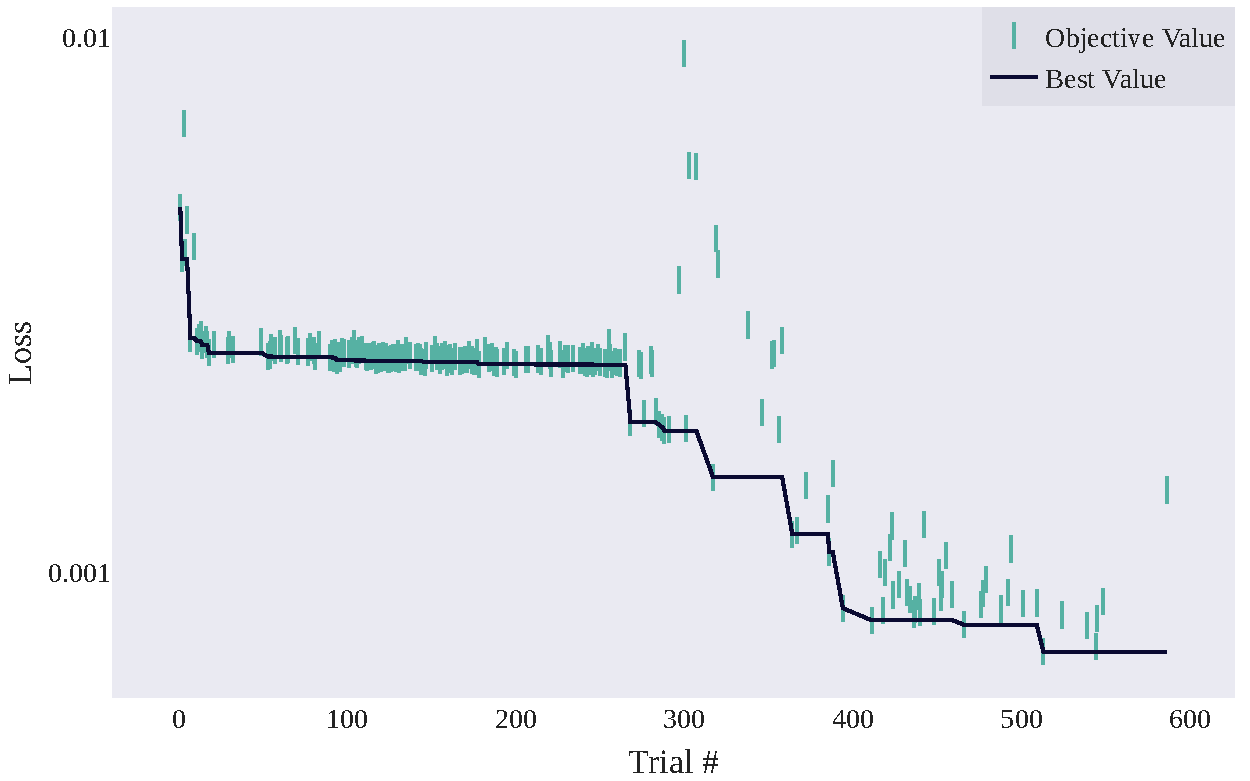
\includegraphics[width=12cm,height=7cm]{images/chapter_3/Optimization_History.pdf}
\caption{Best loss values found during hyper-parameter optimization. The effect of a switch to random sampling and an increase of the pruning threshold can be observed during trials 270 and 310.}
\label{chap3:bestvalues}
\end{figure}

\begin{figure}[htbp]
\centering
\textbf{Loss Value per Epoch for Top 10 Trials}
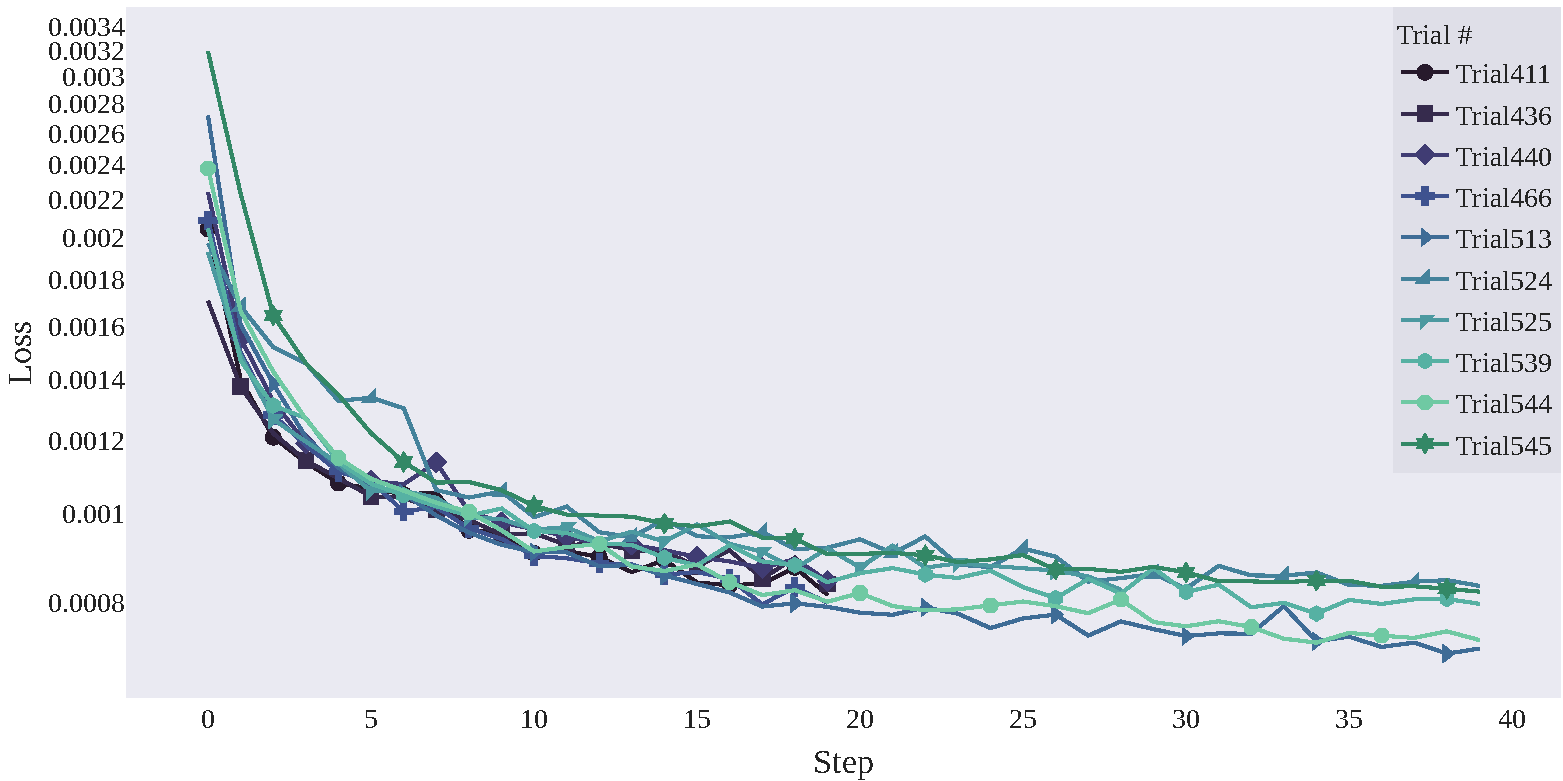
\includegraphics[width=12cm,height=6.5cm]{images/chapter_3/loss_per_training.pdf}
\caption{Loss value per epoch for top 10 trials. Some of the initial 500 trials appear in this list, despite having half the number of epoch steps. The learning curves tend to flatten quickly. Therefore, 20 epoch steps may be a reasonable number for measuring hyper-parameter viability. }
\label{chap3:top10}
\end{figure}


\begin{figure}[t]
\begin{center}
    \textbf{Hyper-Parameters' Loss Correlation}
    \makebox[\textwidth]{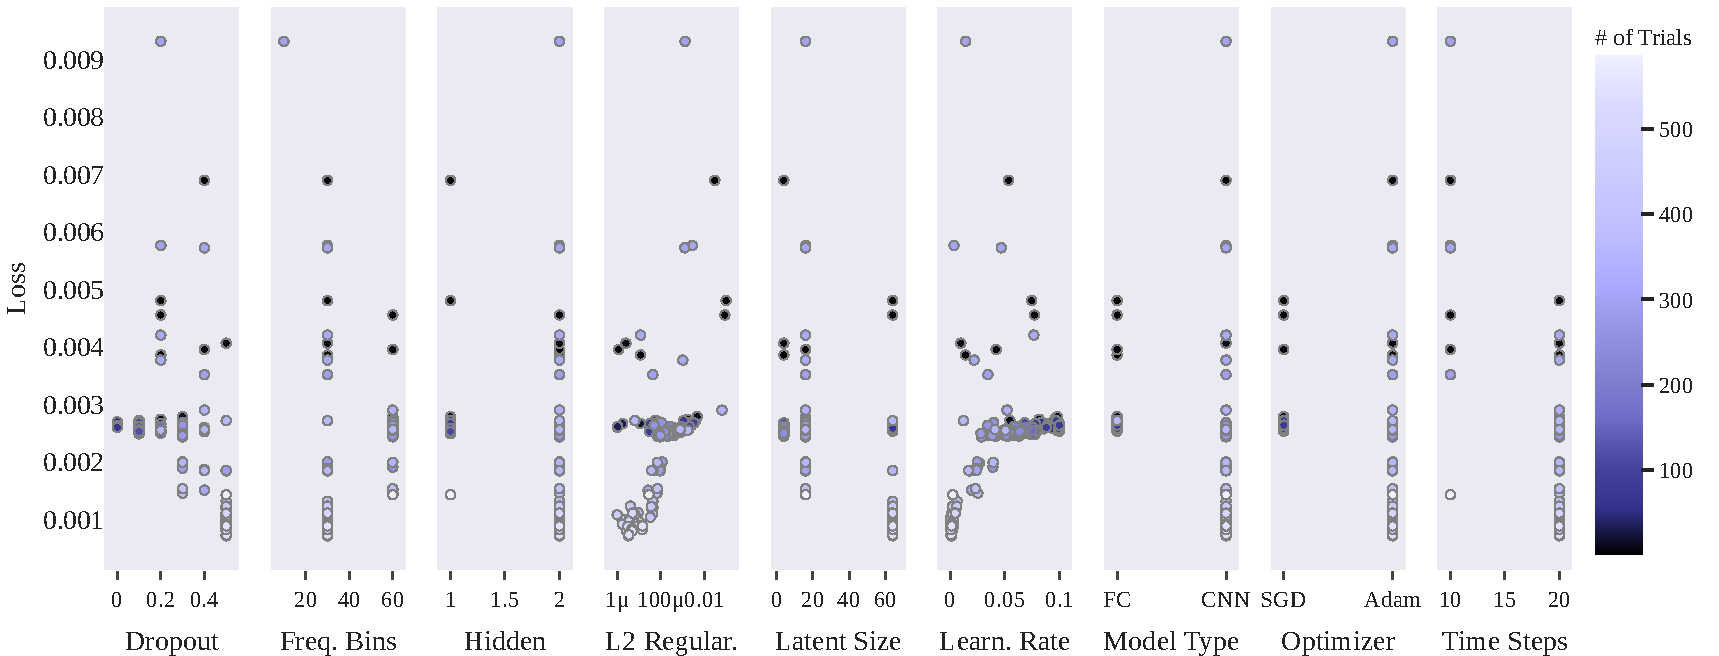
\includegraphics[width=0.95\paperwidth]{images/chapter_3/slice_plot.pdf}}
      \caption{Sliced plot depicting the correlation between hyper-parameters and loss values. The color-scale shows the number of times each parameters has been used in a trial. Our sampling algorithm aims to utilize spaces with higher potential more often. }
    \label{fig:slicegraph}
    \end{center}

\end{figure}
\begin{figure}[h!]
\begin{center}
    \textbf{ Parallel Coordinates of Hyper-Parameter Sets and Loss}
    \makebox[\textwidth]{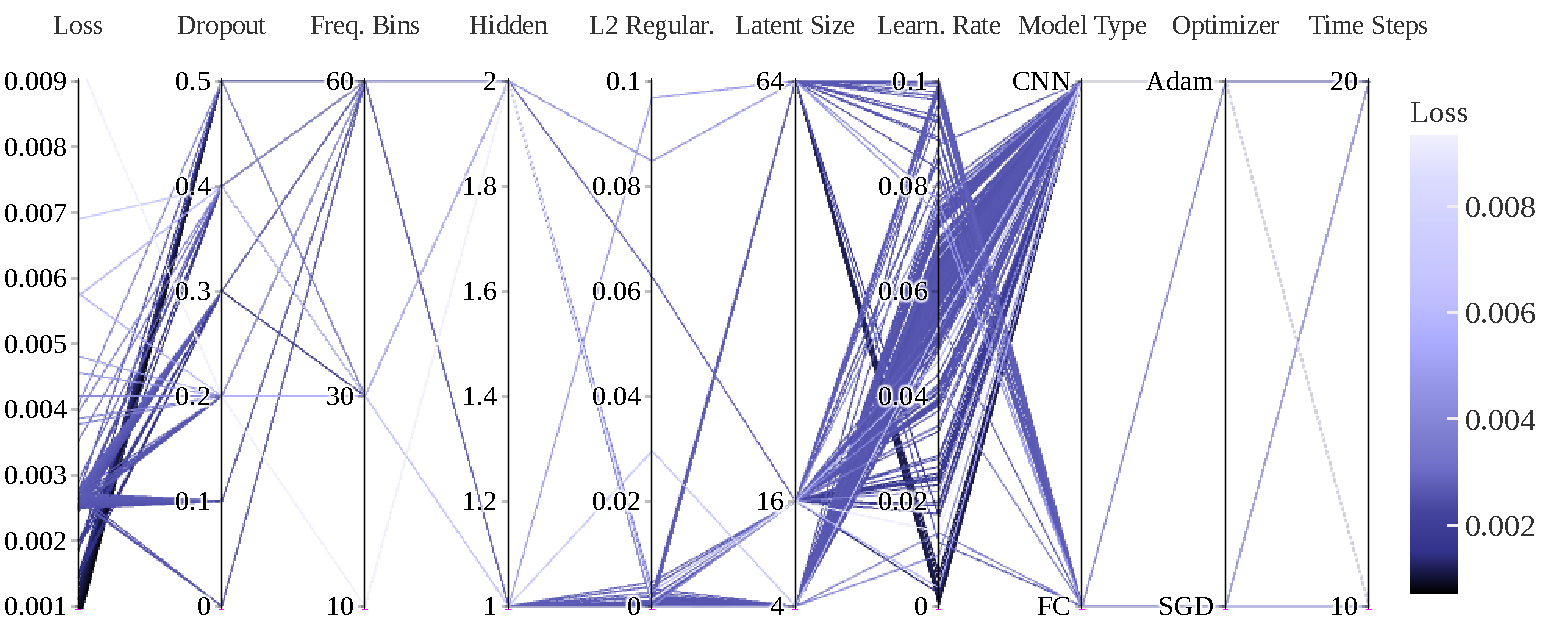
\includegraphics[width=0.9\paperwidth]{images/chapter_3/parallel_coord.pdf}}
      \caption{Not sure if worth keeping. Paths connect hyper-parameters in a set. Path's are colored based on loss value.}
       \label{fig:parallel_coord}
    \end{center}
   
\end{figure}

We depict the correlation of parameter values with trial results in figures~\ref{fig:slicegraph} and~\ref{fig:parallel_coord}. We extract a more concrete measurement of hyper-parameter influence using Hutter et al.'s fANOVA importance evaluator~\cite{hutter2014efficient}. We limit this analysis to 500 trials with 20 epochs. The results of this estimation are depicted in figure~\ref{chap3:param_importance}. Contrasting the results of the fANOVA evaluator with figure~\ref{fig:slicegraph}, we notice several issues. Notably, the importance of 0 is attributed to \enquote{Model Type} and \enquote{Optimizer} parameters, despite a visible difference depicted in the slice-graph. This may be due to the imbalanced sampling of the hyper-parameter space, prompted by our greedy search in place of random sampling. Another possible cause is the \enquote{averaging} of loss results regardless of variance: For example, the slice-graph depicts CNN models as having the best and worst results while FC models are reliably average; Making the fANOVA's 0 importance attribution logical, but not optimal when we are strictly looking for the best models. 

\begin{figure}[t!]
\centering
\textbf{Estimated Parameter Importance}
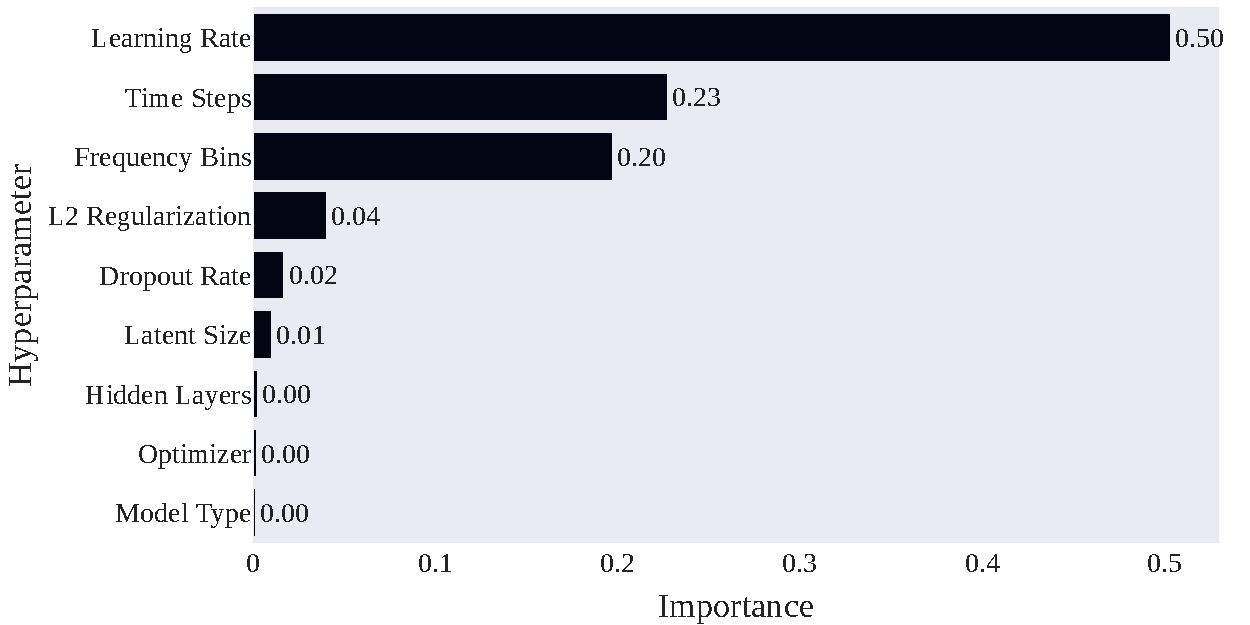
\includegraphics[width=14cm,height=7cm]{images/chapter_3/ParameterImportances_final.pdf}
\caption{The parameters' estimated importance in determining the outcome of trials. Specifications of the spectrogram seem to affect the outcome more so than the model's configuration. We attribute the contrast between the results here and those in figure~\ref{fig:slicegraph} and~\ref{fig:parallel_coord} to the irregular rate of sampling from the hyper-parameter space.}
\label{chap3:param_importance}
\end{figure}

\subsection{Possible Explanation for Embedding Ear's Effectiveness}
How well does our best autoencoder work? What happens if we create a feedback loop where a decoded spectrograms are fed through the network again? 
\begin{figure}[h!]
\centering
\textbf{Recursive Recreation of Drums and Synthetic Noise}\par\medskip
\makebox[\linewidth][c]{%
\begin{subfigure}[b]{.6\textwidth}
\centering
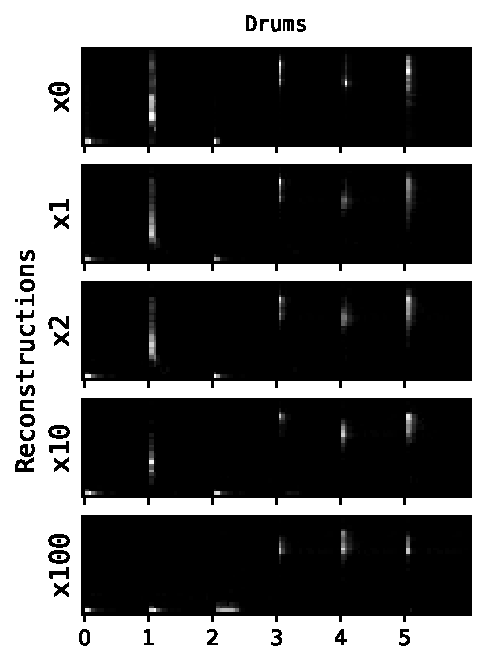
\includegraphics[width=.95\textwidth]{images/chapter_3/Drums_reacreation.pdf}
% \caption{a test subfigure}
\end{subfigure}%
\begin{subfigure}[b]{.6\textwidth}
\centering
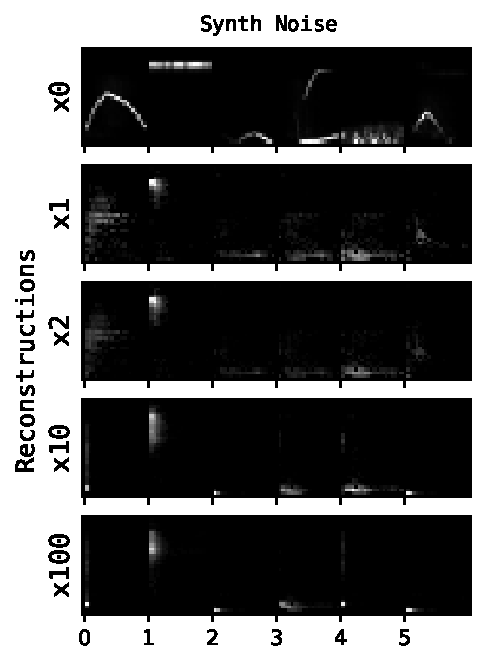
\includegraphics[width=.95\textwidth]{images/chapter_3/Synth Noise_reacreation.pdf}
% \caption{a test subfigure}
\end{subfigure}%
}\\
\caption{We concatenate 6 spectrograms for drum and synthetic noise groups. We recursively encode and decode these spectrograms and display the results. The first row depicts the unaltered spectrograms. We display the results after 1, 2, 10 and 100 recursive recreations. We see that drum spectrograms retain their original form better than synthetic noise.}
\label{fig:recreations}
\end{figure}

We recursively run the autoencoder on new sounds and display the results in figure~\ref{fig:recreations}. The results are displayed for 1, 2, 10 and 100 recursions. Spectrograms belonging to percussive groups retain their unique characteristics for a few time steps, while details in most synthetic noise spectrograms are quickly dissipated. A major point of concern here is that recursively recreated synthetic noise spectrograms tend to take on drum characteristics. This is possibly prompted by our encoder only having been exposed to drums sounds prior.  Yet it is possible that the \enquote{confusion} demonstrated by the encoder after the initial reconstruction leads to embedding of familiar sounds being distinguishable from those unseen. If correct, this approach may have beneficial implications in addressing the aforementioned OSR problem.  


\subsection{Feature Extraction}
\label{fig:embedding_FE}
\begin{table}[htbp!]
\centering
\begin{tabular}{|p{6cm}|p{6cm}|}
\hline
Hyper-Param. & Value  \\ \hline
Model Type      &  CNN  \\ \hline
Optimizer       & Adam  \\ \hline
Hidden Layers   & -  \\\hline
Learning Rate   &  0.001145\\ \hline
Frequency Bins & 30 \\ \hline
Time Steps & 20 \\ \hline
Latent Size & 64 \\ \hline
Regularization & 3.25^{-6}\\ \hline
Dropout Rate & 0.5 \\ \hline
\end{tabular}
\caption{Top performing hyper-parameter set}
\label{table:best_params}
\end{table}
\begin{figure}[h!]
\centering
\textbf{2 Dimensional Projection of Latent Variables}\par\medskip
 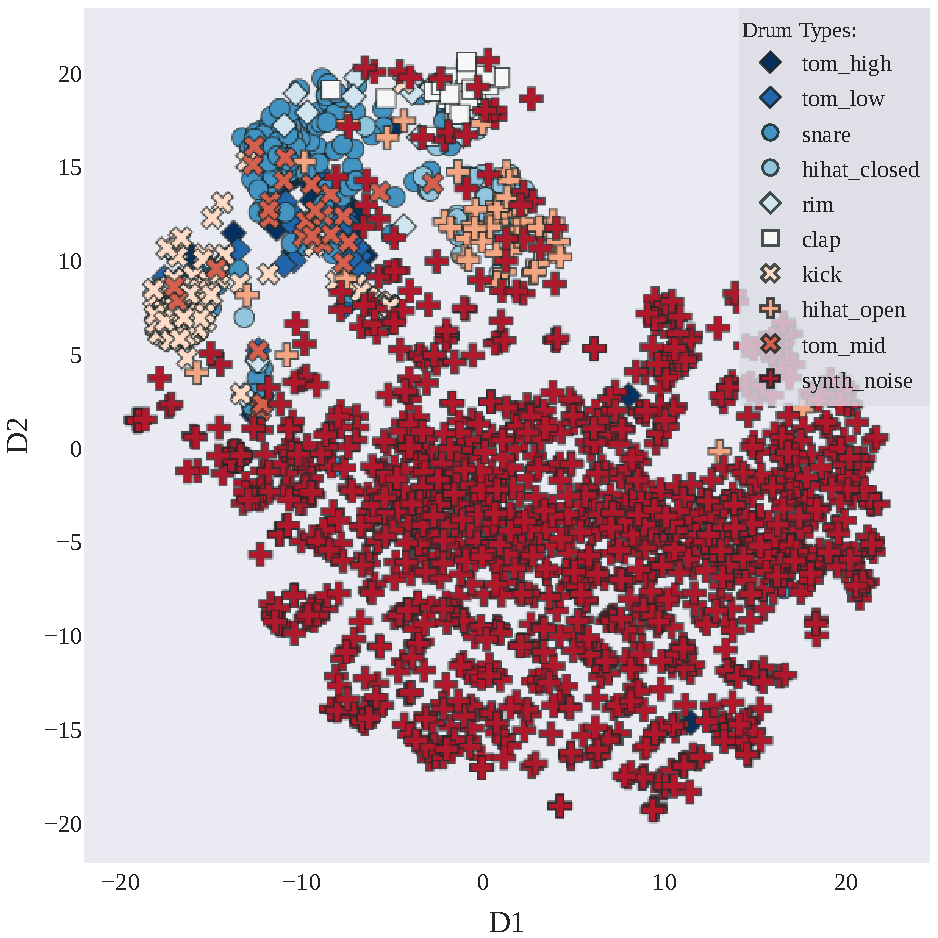
\includegraphics[width=0.90\linewidth]{images/chapter_3/t-SNE_2d.pdf}
\caption{Projection of an embedding model's low dimensional encoding on to a 2D plane. We implemented interactions for these graphs for manual inspection of samples.}
\label{fig:2d_tsne}
\end{figure}

\begin{figure}[htbp!]
\centering
\textbf{3D t-SNE Projection}\par\medskip
\mbox{\subfloat[]{\label{subfig:1} \fbox{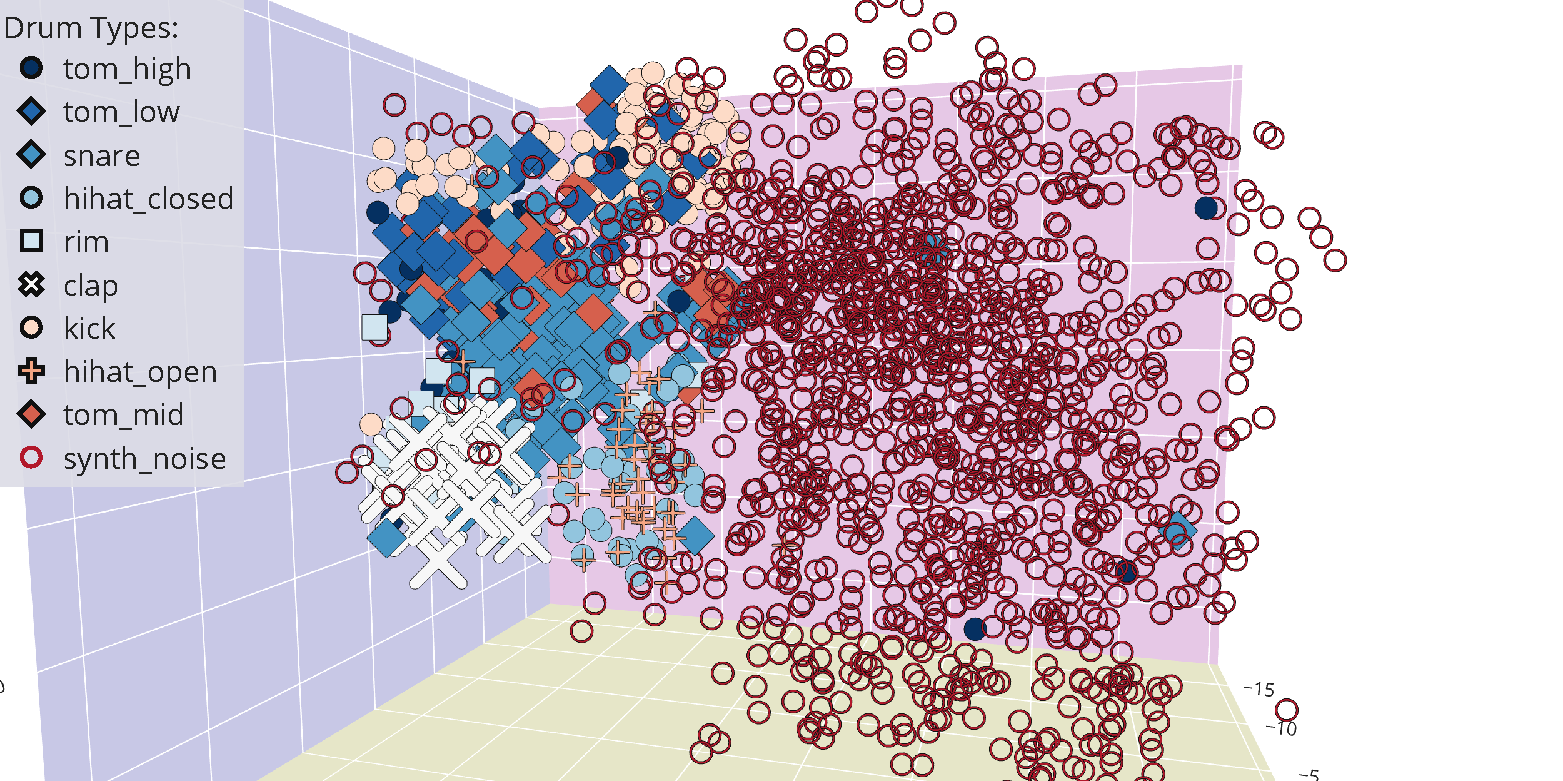
\includegraphics[width=14cm,height=6.8cm]{images/chapter_3/3d_t-SNE_symdrum_type_cam0.pdf}}}}

\mbox{\subfloat[]{\label{subfig:2} \fbox{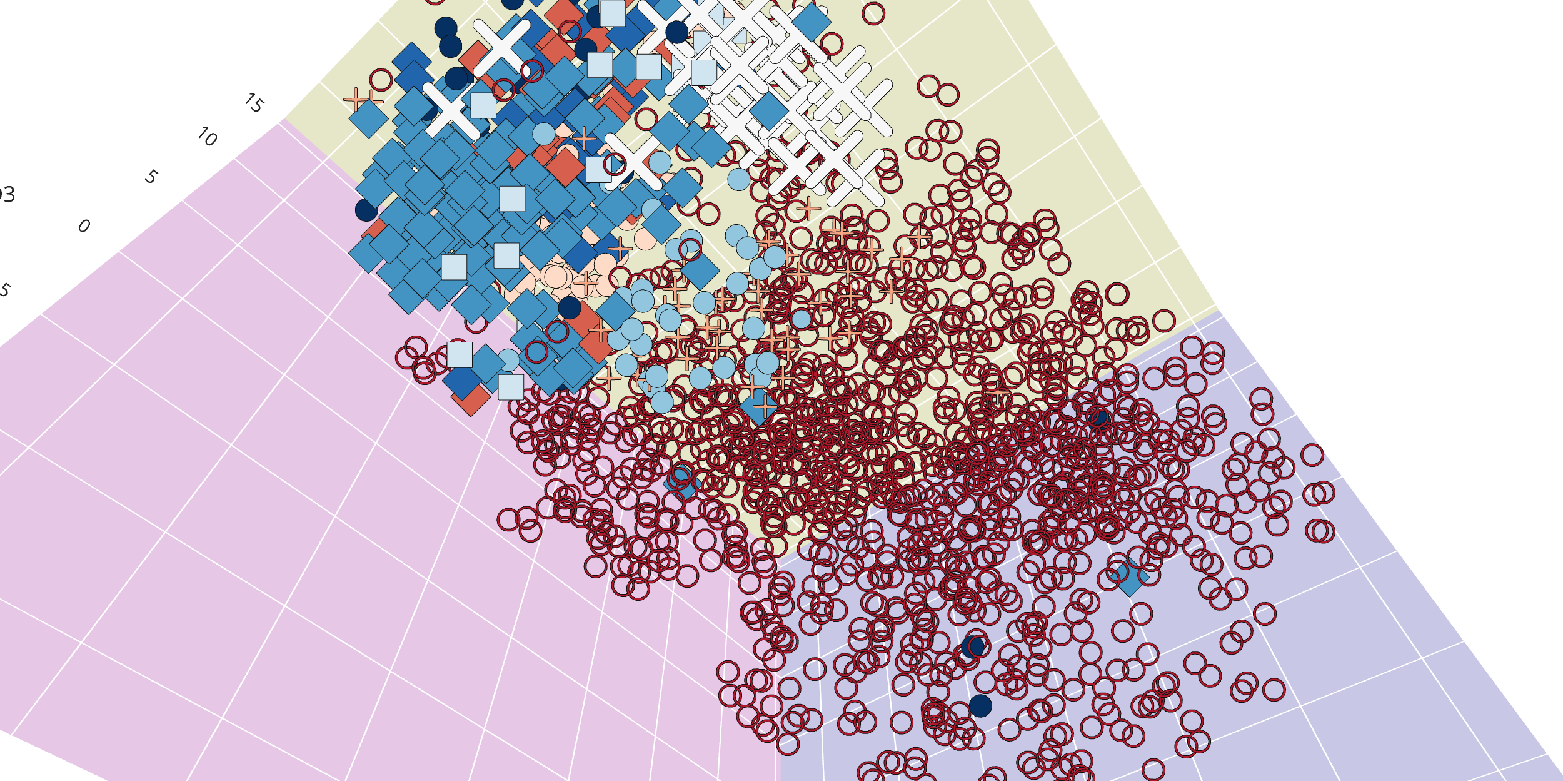
\includegraphics[width=14cm,height=6.8cm]{images/chapter_3/3d_t-SNE_symdrum_type_cam3.pdf}}}}

\fbox{\mbox{\subfloat[]{\label{subfig:2} 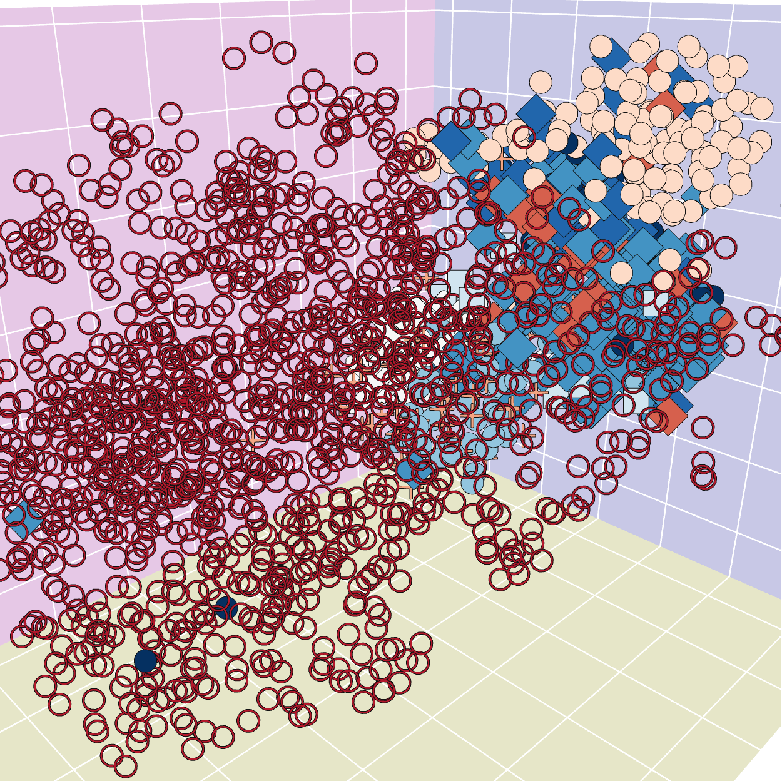
\includegraphics[width=5cm,height=5cm]{images/chapter_3/3d_t-SNE_symdrum_type_cam1.pdf}}}
\mbox{\subfloat[]{\label{subfig:2} 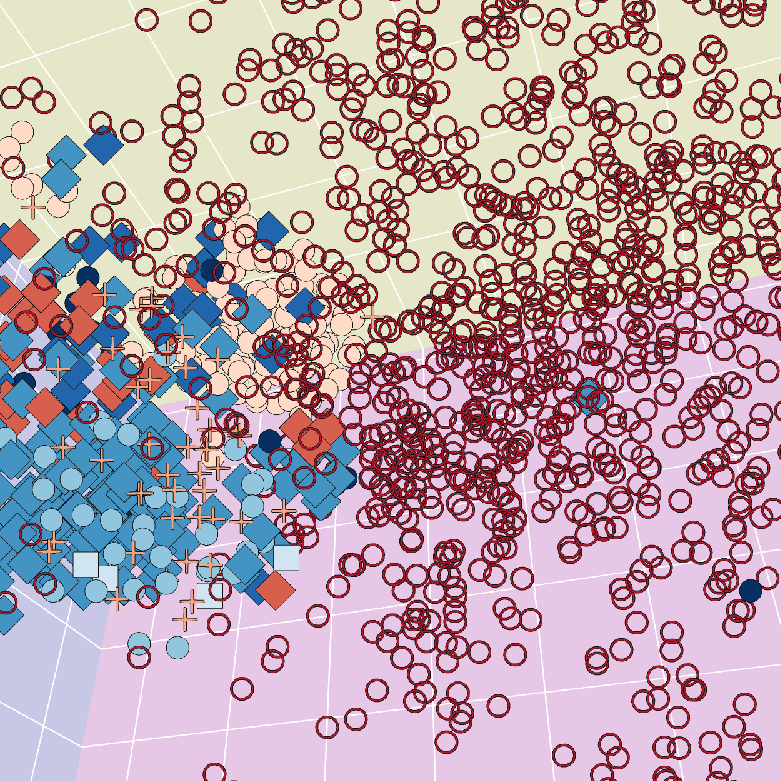
\includegraphics[width=5cm,height=5cm]{images/chapter_3/3d_t-SNE_symdrum_type_cam2.pdf}}}}
\caption{Our feature projections and interactive graphs can also be done in 3D}
\label{fig:3d_tsne}
\end{figure}
To better understand the delineation potential of the encoded features,  we trained an autoencoder with our top performing hyper-parameter set, shown in table~\ref{table:best_params}. We used \%80 of MixedDB to train the model for 200 epochs. Using this model, we encoded the remaining \%20 and approximately 1000 randomly selected sounds from NoiseDB into 64 dimensions. These 64-dimensions were then projected onto a 2 or 3-dimensional plane using t-SNE. Referring to~\hypref{Decision.1} and~\hypref{Decision.2} to define our expectation of a useful encoder, we expect the drum sounds to be clustered together, with the majority of the synthetic noise sounds appearing away from these clusters. Our projections confirm that this is the case. We are most interested in synthetic noise sounds which appear within or near these clusters. Do these synthetic noise sounds have drum like characteristics?\\ 

To test this, we implemented interactive graphs identical to those depicted in figures \ref{fig:2d_tsne} and~\ref{fig:3d_tsne}; These graphs allow for interactions such as playing the samples (by hovering the cursor on-top) and movement of the scene camera for a closer look at clusters.  Manual inspection reveals a noticeable, positive correlation between distance and similarity of a synthetic sound to a drum cluster. Divergences from the envelope features expected from drums are a common point of failure. A noticeable case was a synthetic noise resembeling a \emph{reverse} kick drum within the kick cluster. While encouraging, we hypothesize that more specialized forms of encoding or addition of other features are needed for reducing the frequency of errors and strengthening this correlation.

We see possible benefits in a mixture of envelope features with embedding features. In Section~\ref{chap3:mixed_ear_models}, we analyze the potential gains in using both features for extraction of drum-like sounds from synthetic noise. 

\end{document}